\begin{frame}{Nintendo Entertainment System (NES)}
	\begin{columns}
		\begin{column}{0.32\textwidth}
			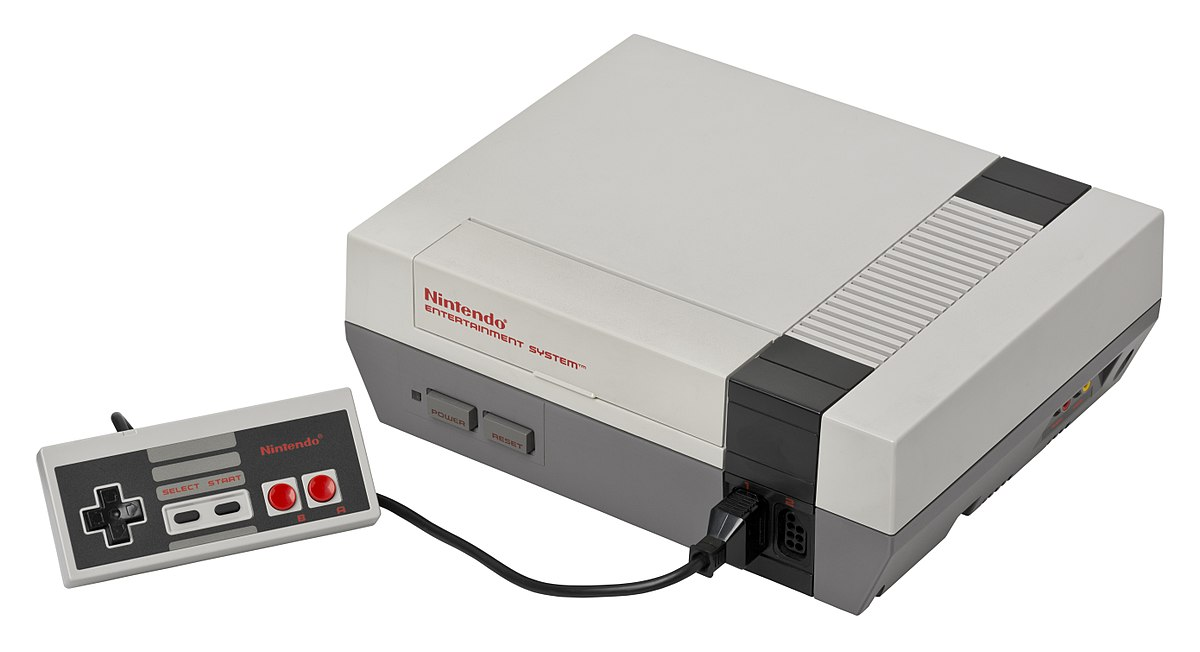
\includegraphics[width=\textwidth]{nes}
			
			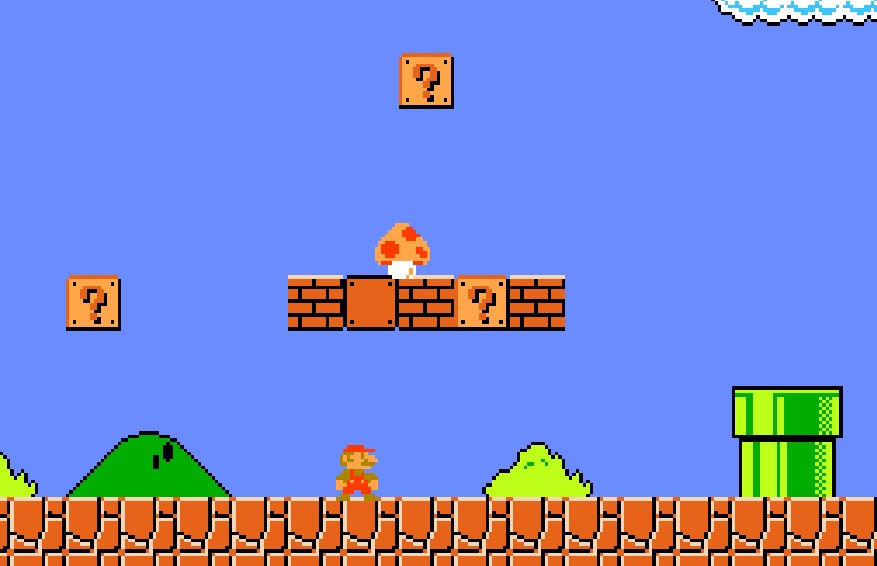
\includegraphics[width=\textwidth]{supermario}
		\end{column}
		\begin{column}{0.64\textwidth}
			\begin{itemize}
				\pause\item Released in \textbf{1983}
				\pause\item Sold as the \textbf{Famicom} (Family Computer) in Japan
				\pause\item Nearly \textbf{62 million} units sold worldwide
				\pause\item Biggest selling game: \textbf{Super Mario Bros}
				\pause\item Credited with reviving the games industry after the \textbf{video game crash} of the early 80s
			\end{itemize}
		\end{column}
	\end{columns}
\end{frame}

\begin{frame}{Nintendo Entertainment System (NES)}
	\begin{columns}
		\begin{column}{0.32\textwidth}
			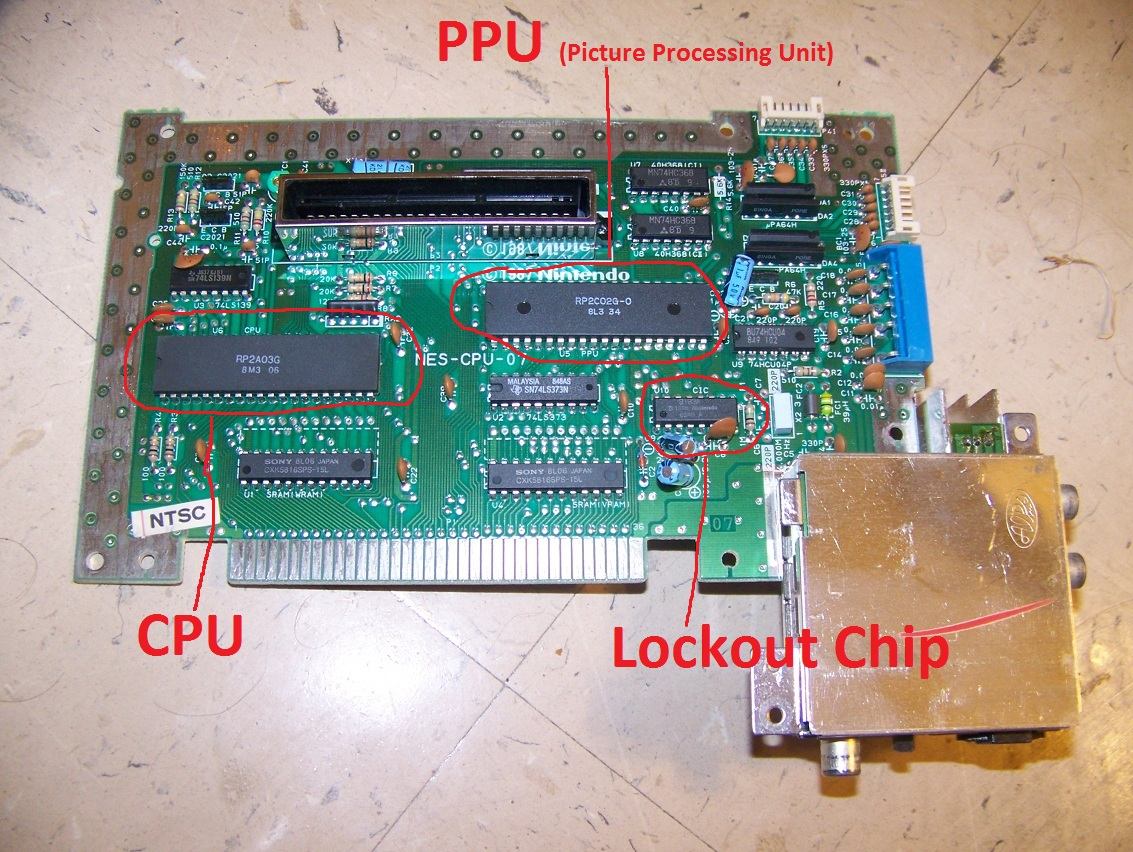
\includegraphics[width=\textwidth]{nes_motherboard}
		\end{column}
		\begin{column}{0.64\textwidth}
			\begin{itemize}
				\pause\item CPU: Ricoh 2A03 (closely based on MOS 6502)
				\pause\item Custom \textbf{Picture Processing Unit (PPU)}
				\pause\item RAM: 2 kilobytes
				\pause\item Screen resolution: 256 $\times$ 240
			\end{itemize}
		\end{column}
	\end{columns}
\end{frame}
